\documentclass{article}
\usepackage[utf8]{inputenc}
\usepackage{mathtools}
\usepackage{amsthm}
\usepackage{amsmath}
\usepackage{amssymb}
\usepackage{marvosym}
\usepackage{hyperref}
\usepackage{fullpage}
\usepackage{xcolor}
\usepackage[labelfont=bf]{caption}
\hypersetup{
    colorlinks,
    linkcolor={red!50!black},
    citecolor={blue!50!black},
    urlcolor={blue!80!black}
}

%\usepackage{babel}
%\include{commands}

\providecommand{\abs}[1]{\lvert#1\rvert}
\providecommand{\norm}[1]{\lVert#1\rVert}
\providecommand{\inprod}[1]{\langle#1\rangle}
\providecommand{\set}[1]{\{#1\}}
\providecommand{\seq}[1]{<#1>}
\providecommand{\bydef}{\overset{\text{def}}{=}}

\providecommand{\R}{\ensuremath{\mathbb{R}}}
\providecommand{\vx}{\vec{x}}
\providecommand{\vy}{\vec{y}}
\providecommand{\vz}{\vec{z}}

\providecommand{\mA}{\mat{A}} 

\renewcommand{\vec}[1]{\ensuremath{\boldsymbol{#1}}}
\providecommand{\mat}[1]{\ensuremath{\boldsymbol{#1}}}

\providecommand{\vsig}{\vec{\sigma}}
\providecommand{\s}{\sigma}

\newcommand{\explain}[2]{\overset{\text{\tiny{#1}}}{#2}} %for i.i.d etc
\renewcommand{\P}{\mathbb{P}} %% for probabilities
\newcommand{\E}{\mathbb{E}} %% for expectations

\newcommand{\gauss}[2]{\mathcal{N}\left( #1,#2 \right)} %% for Gaussian distribution
\newcommand*\diff{\mathop{}\!\mathrm{d}} %for dx
\newcommand{\Tr}{\mathrm{Tr}}

\newtheorem{lemma}{Lemma}

\theoremstyle{definition}

\newtheorem{definition}{Definition}
\newtheorem{fact}{Fact}
\newtheorem{question}{Question}
\newtheorem{subquestion}{Question}[question]

\usepackage{comment}

\def\showsolutions{1}
\ifnum\showsolutions=1
\newenvironment{solution}{\color{blue}{\textbf{Solution \arabic{question}.\arabic{subquestion}:}\smallskip\newline}}{}
\else
\excludecomment{solution}
\fi


\allowdisplaybreaks
\setlength{\parindent}{0pt}

\title{CS 229br Foundations of Deep Learning: Homework 0}

\author{Gustaf Ahdritz \and Boaz Barak \and Gal Kaplun}
\begin{document}
\date{}
\maketitle{}

This homework should be done \emph{before} the semester starts, and would need to be submitted as part of the form to apply for the course. Given limited teaching resources, we will need to cap the number of admitted students. However, we hope that you will still enjoy working on this problem set, even if we are not able to offer you a seat. When working on these problem sets, feel free to use any book or online resource to brush up on topics. We do expect from you not to try just search the concrete question and copy the answer, but rather learn enough about the topic that you can understand it. In fact, being able to search up and learn on your own will be an important skill for succeeding in this course. 

\medskip 
{\color{red} \textbf{Submission instructions:} Use the \href{https://forms.gle/gjXbdCVbqxRVu6Bj6}{Google Form} to submit your solution as two PDF files. For the Theory part, type up your solutions using \LaTeX\ using the provided template. For the programming part, submit a pdf of your jupyter notebook with the required code, plots, and responses.}

\medskip
This course will require you to train deep networks using a framework such as PyTorch, but we will not teach those skills (though teaching fellows are always happy to give out pointers).  Some good resources include:


\begin{itemize}
    \item \href{https://pytorch.org/tutorials/beginner/deep_learning_60min_blitz.html}{60-min blitz} Pytroch tutorial
    \item \href{https://pytorch.org/tutorials/beginner/nn_tutorial.html}{Beginner NN Pytorch tutorial}

    \item For a more in-depth understanding of automatic differentiation, pytorch, and tensors go through Sasha Rush's \href{https://minitorch.github.io/}{minitorch}. You can also do Sasha's \href{https://github.com/srush/Tensor-Puzzles}{Tensor puzzles},  \href{https://github.com/srush/GPU-Puzzles}{GPU puzzles}, and \href{https://github.com/srush/Autodiff-Puzzles}{Auto differentiation puzzles}. (If you do solve some of these puzzles, please post your stats---how many puzzles you solved from each sequence---on the course's Slack board!)

    \item Another good  resource for deep learning self-study is \href{https://dataflowr.github.io/website/}{Dataflower}
    
\end{itemize}

We strongly suggest you go over at least some of these resources \emph{before} the semester begins. This will enable you to get much more out of CS 229br.


\section*{Pen and paper questions}

(While we recommend \emph{solving} these using pen and paper, you will still need to type up your solution in \LaTeX.)

\begin{question}
Consider the following setting.

\begin{itemize}
    \item For some $w_*\in\mathbb{R}^d$, the distribution $D_{w_*}$ is over pairs $(x,y) \in \mathbb{R}^{d+1}$ such that $x\sim N(0,I_d)$ and $y = \langle x,w_* \rangle + N(0,1)$.

    \item We are considering the regression task, in which we are given $n$ samples $S = \{ (x_1,y_1),\ldots,(x_n,y_n) \}$ drawn independently from $D_{w_*}$, and our goal is to find a function $f:\mathbb{R}^d \rightarrow \mathbb{R}$ that minimizes $\mathbb{E}_{(x,y)\sim D_{w_*}}[ (f(x)-y)^2 ]$. We define this quantity as $\mathcal{L}(f)$.
\end{itemize}
\end{question}

\begin{subquestion}[Generalization bound]
Let $\mathcal{F}$ be a finite set of bounded functions mapping $\mathbb{R}^d$ to $[-B, B]$, for some constant $B>0$. Prove that with probability at least $0.01$ over the choice of $S$, 
\begin{equation*}
    \max_{f\in\mathcal{F}} \left|   \mathcal{L}(f) \;-\; \tfrac{1}{n}\sum_{(x,y)\in S} \left( f(x)-y\right)^2 \right| \leq O\left(\sqrt{\tfrac{\log |\mathcal{F}|}{n}} \right)
\end{equation*}
\textbf{Hint.} See \href{https://www.stat.berkeley.edu/~mjwain/stat210b/Chap2_TailBounds_Jan22_2015.pdf}{link}.  
\end{subquestion}


\begin{solution}
Your solution here
\end{solution}

\begin{subquestion}[Optimization]
In this question we consider the \textit{under-parameterized} setting where $n \gg d$. Let $\mathcal{F}$ be the set $\{ f_w : w\in \mathbb{R}^{d+1} \}$ where $f_w(x) = \langle w,x \rangle$. Assume $\| w_*\|^2=d$, and consider the \textit{stochastic gradient descent} algorithm on $\mathcal{L}$.
For $(x,y)$ and function $f:\mathbb{R}^d \rightarrow \mathbb{R}$, we define $\mathcal{L}_{x,y}(f) = (f(x)-y)^2$, and consider the following algorithm, where $\delta,\eta$ are hyperparameters: 

\begin{itemize}
    \item Let $w_0 \sim N(0,\delta \cdot I_d)$. 
    \item For $t=0,2,\ldots,n-1$ do the following:
        \begin{itemize}
            \item Let $(x,y) \sim D_{w_*}$
            \item Let $w_{t+1} = w_t - \eta \nabla \mathcal{L}_{(x,y)}(f_{w_t})$
        \end{itemize}
\end{itemize}

Prove that, \textit{in expectation}, this algorithm makes progress towards the optimal solution in every iteration. Specifically, prove that there exists some constant $c \in \mathcal{R}$ such that, for any $t$:
\begin{equation*}
    E[\nabla L_{(x_t, y_t)}(f_{w_t})] = c(w_t - w_*)
\end{equation*}

It is possible to use this fact to prove that, in this particular setting, SGD converges to the optimal solution with high probability.
   
\end{subquestion}
    
\vspace{10pt}

\begin{solution}Your solution here
\end{solution}


\begin{subquestion}[Inductive bias]
In this question we consider the \textit{over parameterized} setting where $n\ll d$. We show that in this case gradient descent has a certain bias toward low-norm solutions. Specifically, consider the algorithm above.

\begin{enumerate}

\item Prove that in all steps of stochastic gradient descent above, we maintain the invariant that $w_t \in \mathrm{Span}(w_0,x_0,\ldots,x_{t-1})$ where $(x_i,y_i)$ is the sample drawn in step $i$. 

\item Let $S$ be some set $\{ (x_0,y_0),\ldots, (x_{n-1},y_{n-1}) \}$ in $\mathbb{R}^d$ in ``general position'' ( $\| x_i \|^2\approx d$ for all $i$, $\langle x_i,x_j \rangle^2 = o(\sqrt{d})$ for all $i \neq j$, $|y_i|^2 = O(1)$) and let $w_0 = 0$. Suppose that we run the algorithm on $S$ and that it successfully converges, i.e. $\forall i \leq n, \langle x_i, w_n \rangle = y_i$. Prove that $w_n$ is 

$$\arg\min_{w : \text{ s.t. } \langle x_i, w \rangle = y_i} \| w \|^2$$

Thus, among all possible ``interpolating solutions'' to the training set, the algorithm chooses the one that is smallest in $L_2$ norm.

\end{enumerate}
\end{subquestion}


\begin{solution}
\textbf{Item 1:} Your solution here 


\textbf{Item 2:}  Your solution here
\end{solution}

\section*{Programming questions}

{\color{blue} Submit the results of the programming question - code, plots, and textual explanations - as a separate pdf file }

\begin{question}[Toy image search engine]
Complex classical algorithms often depend on elementary algorithms with well-known properties---think binary search and quicksort---as subroutines. Analogously, state-of-the-art machine learning (ML) pipelines are often built with combinations of ``soft'' pretrained machine learning primitives. Developing a familiarity with the rapidly expanding toolkit of these ML ``building blocks'' will make it easier to read new ML papers and design ML solutions of your own. \\

Over the past couple of years, OpenAI's CLIP has become a popular primitive for a wide range of image-related tasks. In this exercise, we will use CLIP to build a simple text-to-image search tool. \\
    \end{question}

\begin{subquestion}[Setup]
We will need a GPU to train models quickly. If you have an existing GPU setup (\textit{e.g.} via your lab), you can use that. Otherwise, we recommend using a free GPU on Google Colab:
\begin{itemize}
    \item Create a Google Colab notebook
    \item In Runtime $\rightarrow$ ``Change runtime type'' select ``GPU'' as your hardware accelerator. 
\end{itemize}

Note that your session will time out if you leave it unattended for too long. \\

We included a \href{https://colab.research.google.com/drive/1E838sz34fNS2OjsznT_hWIM_eulX4g2x?usp=sharing}{minimal notebook} which trains a 5-layer CNN on CIFAR-10. Make sure you can run this on your GPU (/Colab). It should reach ~85\% test accuracy in ${\sim}$4 minutes. Play around with parameters in this notebook to get a better feeling of training models (try changing the model definition, the batch sizes, the learning rate schedule, the number of train samples, the optimizer, etc). Record any interesting behaviors you notice. \\

(Optional) The network we define has batch normalization layers. Remove these layers and try to train the network. It should still work, but may be more sensitive to choices like initialization, layer widths, and learning rates. If you are interested, we recommend \href{https://arxiv.org/abs/1912.08957} {this survey} on optimization considerations in neural networks. It is an open problem to understand necessary and sufficient conditions that ensure neural networks can be properly optimized with SGD (see the suggestions in the survey---can you replicate their predictions with experiments?) \\
    
Extra Tips:
\begin{itemize}
    \item \href{http://karpathy.github.io/2019/04/25/recipe/}{Practical tips} on training NNs, from Andrej Karpathy.
    \item \href{https://myrtle.ai/learn/how-to-train-your-resnet/}{How to Train Your ResNet} by David Page, walks through the design and debugging process of training a state-of-the-art network. Note the careful experimental design at each stage.
    \item For longer-running training jobs, you may want to create a stand-alone training script instead of running jobs in notebooks.
    \item We highly recommend using \href{http://wandb.ai/}{wandb} (free) to track and log your experiments. For example, we like to use wandb to track train/test errors of models as they train and automatically plot them in the web UI.
    \item You may like \href{https://www.pytorchlightning.ai/}{Lightning} which removes some PyTorch boilerplate.
\end{itemize}
\end{subquestion}

\begin{subquestion}[Comprehension]
Read the first few pages of \href{https://arxiv.org/abs/2103.00020}{the CLIP paper} (at least up to the evaluation section). You may also consult other sources if you wish. In your own words, describe how CLIP works. What kind of data is it trained on? What is the training objective? How does it differ conceptually from simple classifiers like the one we trained in the previous exercise? What can it be used for?
\end{subquestion}

\begin{subquestion}[Search Engine] \label{ques:searchengine}
Install \href{https://github.com/openai/CLIP}{CLIP} (checkpoint ``ViT-B/32'') and \href{https://github.com/facebookresearch/faiss}{Faiss}, a library for efficient vector similarity search. Make sure to take a look at the sample programs in both READMEs. To simplify our computations a little, we'll be using images from the training and validation sets of TinyImageNet, a dramatically shrunken version of the full ImageNet dataset. Download it \href{https://www.image-net.org/}{here}. You'll need to make an account using your Harvard email. \\

As always, the first step is to get hands-on with the data; if there are problems, we'd rather know \textit{before} we spend time trying to optimize our ML pipelines. Manually inspect a handful of images chosen at random from the training and validation sets. Write down some of your observations. What are some things you notice about the images? Do the provided labels correspond well to what you see in the images? What are some limitations of this dataset (even for human ``search engines'')? \\

We'll be implementing search over the validation set. Precompute CLIP embeddings (or ``features'') for each image in the set and store them in a Faiss index. Given a search query (e.g. ``go-kart''), use CLIP to create a text embedding of that query and then use that to search your Faiss index for the top $k=5$ nearest neighbors according to Euclidean distance. The images corresponding to these nearest neighbors are your search results. Remember to take advantage of your GPU. That's it! The algorithm is visualized in \textbf{Figure \ref{fig:search}}.\\

\begin{figure}[h!]
    \centering
    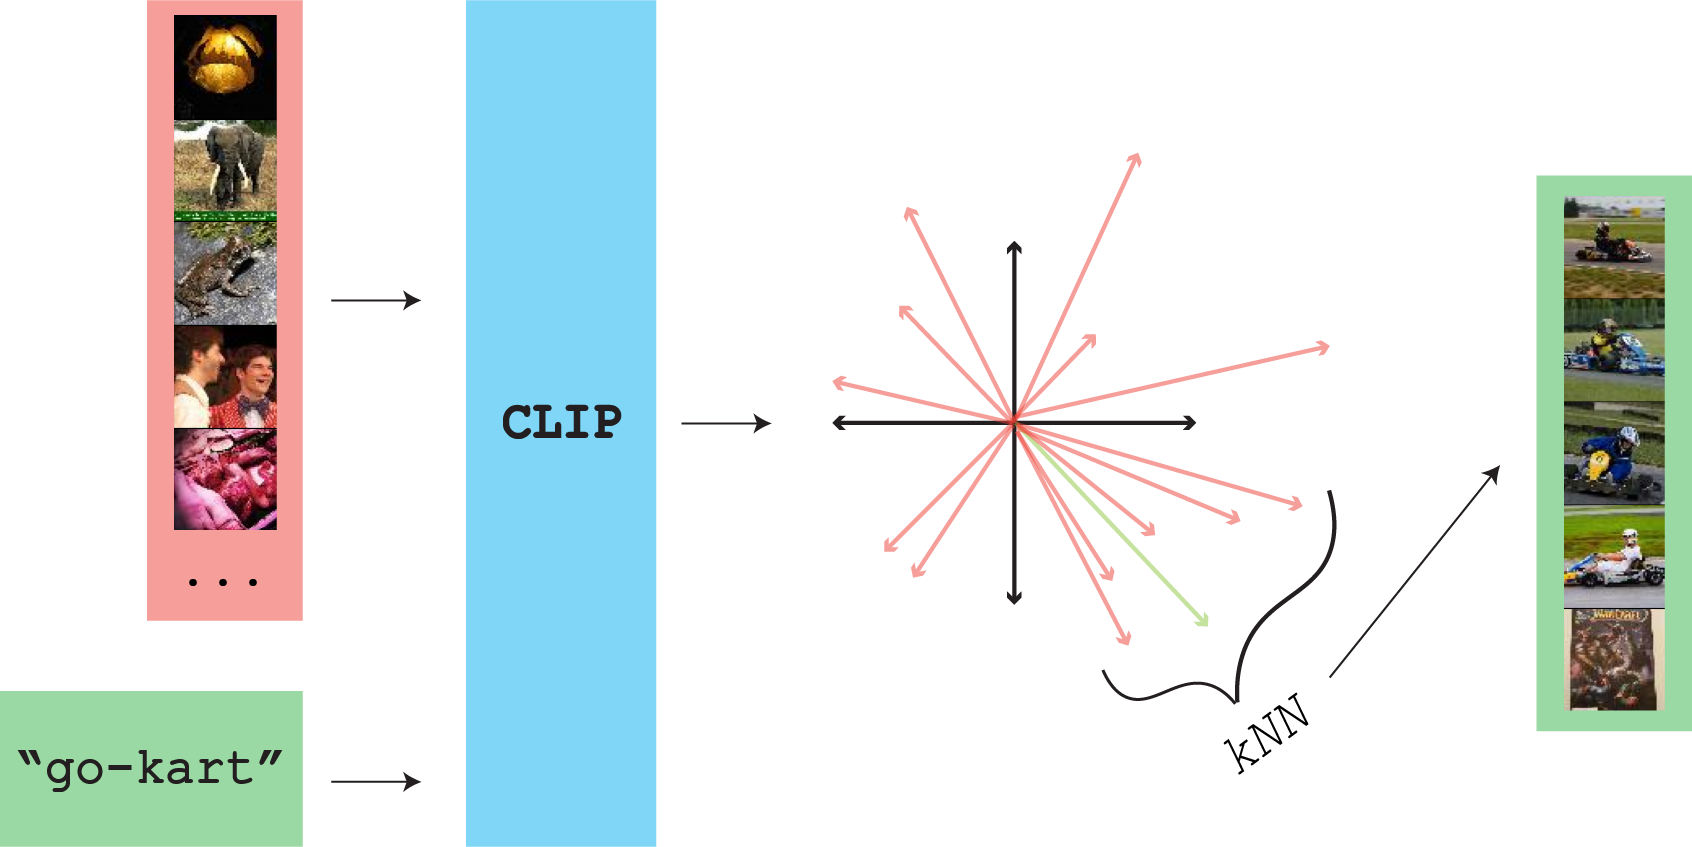
\includegraphics[width=\textwidth]{hw0_fig.png}
    \caption{Our search algorithm. Given a database of (unlabelled) images and a user-specified query, the tool returns the indices of $K=5$ images corresponding to the query. In the visualized example, 4/5 of the returned images actually have the ImageNet label ``go-kart''. Note that real CLIP embeddings are high-dimensional.}
    \label{fig:search}
\end{figure}

Despite its simplicity, this tool is powerful; note that you can search for arbitrary phrases, including e.g. adjectives (it can distinguish between ``a car'' and ``a red car''). Play around with it a little, inspecting the returned images. What kinds of mistakes does it make---do they seem random, or can you understand why they happen? Can you fool it with a mean-spirited query? Evaluate its performance systematically by computing accuracy on each TinyImageNet label in the validation set ((\# hits that match the searched label) / $k$). Report the mean accuracy across all labels as well as your own qualitative observations.
\end{subquestion}

\begin{subquestion}[Improving the search engine]
 CLIP was trained on images much more diverse than the tiny, thematically repetitive images in our dataset. In practice, if we cared enough about this particular style of image, we could robustly improve our search engine by finetuning CLIP on text/image pairs from our own dataset. Since we have limited time, data, and compute, however, we'll be making more modest modifications.

\begin{enumerate}
    \item Since we know that our images probably always come from a small number of categories (our TinyImageNet labels), we could augment images in our database using metadata from a classifier. Train a classifier (using a simple MLP or any other architecture of your choice) to predict the label of an image given its CLIP embedding. Specifically, the output should be a distribution over four labels chosen at random from the set of TinyImageNet labels with training data (this happens to be a subset of all of the labels represented in the validation set). The remaining labels should be grouped together into a single ``other'' label. Use cross-entropy loss. Additionally, be very careful not to backpropagate into CLIP; \texttt{detach} all CLIP vectors before you feed them to your classifier, ensuring that you only train the parameters of the classifier itself. In other words, CLIP should be ``frozen'' for this training run. For the purposes of this problem, there's no need to actually incorporate classifier predictions into your search tool; training the classifier is enough. Again, we recommend tracking your classifier's validation set accuracy across the different labels using \texttt{wandb}. Submit your code and a plot of your classifier's validation set accuracy over time.
    \item In Question~\ref{ques:searchengine}, you'll have noticed that your search engine's performance is much worse on some labels than others. Suppose that you have reason to believe that some of these low-accuracy queries are particularly important; let's say \textit{e.g.} you think your users will be enthusiastic about the verbatim query ``scorpion,'' which currently has low accuracy. In such cases, you might consider manually intervening. We have training data for ``scorpion,'' and, as we have argued, that training data is more likely to resemble validation set scorpions than the images CLIP was trained on. Think about how we can use this training data to improve corresponding queries. One simple approach is to train an MLP using SGD to map the single CLIP text query to a query more closely aligned with the CLIP image embeddings of the training data. This has the advantage of not requiring much thought on our part. We encourage you to try this; by passing your low-accuracy ImageNet label CLIP queries through bespoke MLPs, you'll be able to improve accuracy to $>= 0.8$. \\
    
    A common pitfall, however, is applying ML where it isn't strictly needed, creating solutions that are more opaque and therefore difficult to maintain than necessary. Can you think of a simple way to use the CLIP training image embeddings for a particular label to create a better query vector for that label without training a model?
\end{enumerate}
   
\end{subquestion}



 



\end{document}
